\chapter{Algorithm}

\tikzstyle{decision} = [diamond, align=center, draw=black]

\tikzstyle{block} = [rectangle, minimum width=2.5cm, minimum height=1cm, align=left, draw=black]


%\begin{figure}
%\centering
%\resizebox{\textwidth}{!}{
%\begin{tikzpicture}[
%    triangle/.style = {regular polygon, regular polygon sides=3 }
%]
%	\pgfmathsetmacro{\px}{0}
%	\pgfmathsetmacro{\py}{0}
%	\pgfmathsetmacro{\tx}{0}
%	\pgfmathsetmacro{\ty}{-4}
%	\pgfmathsetmacro{\treex}{10}
%	\pgfmathsetmacro{\treey}{0}
%	
%\node [circle, draw, fill=blue!20] (a) at (\px, \py) [minimum size=0.5cm] {};	
%\node [rectangle, draw, fill=blue!20] (b) at (\px, \py-2) [minimum size=0.5cm] {};
%\node (c) at (\px, \py-3) {Pattern Graph};
%\draw (a)--(b);
%
%
%\node [circle, draw, fill=red!20] (d) at (\tx, \ty) [minimum size=0.5cm] {};	
%\node [rectangle, draw, fill=red!20] (e) at (\tx, \ty-2) [minimum size=0.5cm] {};
%\node [triangle, draw, fill=red!20] (f) at (\tx+1.732, \ty-1) [minimum size=0.5cm] {};
%\node (g) at (\tx, \ty-3) {Target Graph};
%\draw (d)--(e);
%\draw (d)--(f);
%\draw (e)--(f);
%
%\draw (\treex, \treey)--(\treex, \treey-2);
%\draw (\treex, \treey)--(\treex-3.5, \treey-2);
%\draw (\treex, \treey)--(\treex+3.5, \treey-2);
%\node [circle, draw, fill=blue!20] at (\treex-3.8, \treey-2.5) [minimum size=0.5cm] {};
%\node [circle, draw, fill=red!20] at (\treex-3.2, \treey-2.5) [minimum size=0.5cm] {};
%
%\node [circle, draw, fill=blue!20] at (\treex-0.3, \treey-2.5) [minimum size=0.5cm] {};
%\node [triangle, draw, fill=red!20] at (\treex+0.3, \treey-2.6) [minimum size=0.5cm] {};
%
%\node [circle, draw, fill=blue!20] at (\treex+3.2, \treey-2.5) [minimum size=0.5cm] {};
%\node [rectangle, draw, fill=red!20] at (\treex+3.8, \treey-2.5) [minimum size=0.5cm] {};

%
%\draw (\treex-3.5, -3)--(\treex-2.625, \treey-4.5);
%\draw (\treex-3.5, -3)--(\treex-4.375, \treey-4.5);
%\draw (\treex, -3)--(\treex-0.875, \treey-4.5);
%\draw (\treex, -3)--(\treex+0.875, \treey-4.5);
%\draw (\treex+3.5, -3)--(\treex+2.625, \treey-4.5);
%\draw (\treex+3.5, -3)--(\treex+4.375, \treey-4.5);
%
%\node [rectangle, draw, fill=red!20] at (\treex-4.075, \treey-5) [minimum size=0.5cm] {};
%\node [rectangle, draw, fill=blue!20] at (\treex-4.675, \treey-5) [minimum size=0.5cm] {};
%\node [rectangle, fill=green] at (\treex-4.45, \treey-5.7) [minimum width=1.8cm, minimum height=0.3cm]{};
%
%\node [rectangle, draw, fill=blue!20] at (\treex-2.925, \treey-5) [minimum size=0.5cm] {};
%\node [triangle, draw, fill=red!20] at (\treex-2.325, \treey-5.1) [minimum size=0.5cm] {};
%
%\node [rectangle, draw, fill=blue!20] at (\treex-1.175, \treey-5) [minimum size=0.5cm] {};
%\node [circle, draw, fill=red!20] at (\treex-0.575, \treey-5) [minimum size=0.5cm] {};
%
%\node [triangle, draw, fill=red!20] at (\treex+1.175, \treey-5.1) [minimum size=0.5cm] {};
%\node [rectangle, draw, fill=blue!20] at (\treex+0.575, \treey-5) [minimum size=0.5cm] {};
%
%\node [rectangle, draw, fill=red!20] at (\treex+2.925, \treey-5) [minimum size=0.5cm] {};
%\node [rectangle, draw, fill=blue!20] at (\treex+2.325, \treey-5) [minimum size=0.5cm] {};
%
%\node [circle, draw, fill=red!20] at (\treex+4.675, \treey-5) [minimum size=0.5cm] {};
%\node [rectangle, draw, fill=blue!20] at (\treex+4.075, \treey-5) [minimum size=0.5cm] {};
%
%\node at (\treex, \treey-6) {Search Space Tree};
%\end{tikzpicture}
%%}
%\caption{State space of subgraph isomorphism search algorithms. Vertices with the same shape may be matched to each other, while vertices with different shapes have incompatible labels. The green bar denotes the only search path that leads to a successful subgraph isomorphism. Source: \cite{RIalgorithm}}
%\label{fig:statespace}
%\end{figure}




\section{Baseline: ndSHD2}
In our research we will extend existing work on node disjoint subgraph isomorphism. In the literature we found two existing concrete algorithms: Xiao's algorithm `ndSHD2'\cite{XIAONODEDISJOINT} and Lingas algorithm\cite{LINGAS2009464}. We choose to adapt Xiao's algorithm ndSHD2 as baseline over Lingas because it is easier to understand (thus easier to improve, saving valuable research time) and includes methods for vertex-on-vertex mapping. In comparison, Lingas' algorithm suggests attempting their edge-path mapping strategy on every possible vertex-on-vertex mapping. We will adapt Xiao's algorithm to compute paths on-the-fly instead of beforehand to avoid the exponential space requirement.

To understand ndSHD2 better, let us first examine what the output is supposed to be. The algorithm should, given two graphs, not just indicate whether the latter graph is a subgraph homeomorphism of the former, but also indicate what subgraph homeomorphism that is. More formally, we need to solve the \textit{certification} problem rather than the \textit{decision} problem. This certification indicates to which target graph vertex each source graph vertex is mapped and to which target graph path each source graph edge is mapped such that the entire mapped source graph is a subgraph of the target graph. This is what we will from now on refer to as the \textbf{mapping}.

\begin{algorithm}[H]
\SetAlgoLined
\textbf{Inputs: } the current matching state $s$, the current node compatibility matrix $M$, the current independent path matrix $R$\\
\textbf{Outputs: } \textit{found}, indicating whether a valid homeomorphism has been found.\\
\If{$s$ is dead state} {
	\Return false\;
} \ElseIf {$s$ is complete} {
	\Return true\;
}

$found \longleftarrow false$

 initialization\;
 \While{$!found \land \exists$ valid node/edge-path mapping pair}{
  $m \longleftarrow GetNextNodePair()$\tcp*[h]{$m \longleftarrow GetNextEdgePathPair()$}\;
  $s' \longleftarrow BackupState(s)$\; 
  $NodeMap_s \longleftarrow NodeMap_s \cup \{m\}$\tcp*[h]{$EdegePathMap_s \longleftarrow EdgePathMap_s \cup \{m\}$}\;
  $Refine(M, R)$\;
  $found \longleftarrow ndSHD2(s, M, R)$\;
  \If{found} {
  	\Return true\;
  }
  $s \longleftarrow RecoverState(s')$\;
 }
 \Return false\;
 \caption{ndSHD2}
 \label{algorithm:ndSHD2}
\end{algorithm}

ndSHD2 Is shown in Algorithm \ref{algorithm:ndSHD2}. It is a form of depth first search in a partial mapping search space that attempts- and backtracks vertex-on-vertex mappings and edge-on-path mappings.

In our literature study, we found that the core of many subgraph isomorphism algorithms\footnote{Ullman, VF, VF2, VF2+, VF2++, UI, Fast-ON, L2G, Cheng, QuickSI, GraphQL, ILF, TurboISO, Glassgow, CLF-Match, RI, RI-DS, McGregor, LAD, PathLAD} is a form of similar DFS state space exploration where the states consist of partial vertex-to-vertex mappings. In subgraph isomorphisms, the edge-to-edge mapping is elementary by performing the vertex mapping on the edge source and target to obtain the target edge. With the subgraph homeomorphism algorithm such as Xiao's, an additional mapping from $E_{source}$ to the path set of $G_{target}$ is needed.

The algorithm starts with an empty partial mapping, and starts mapping source graph vertices to target graph vertices. Whenever both vertices of a source graph edge has been matched, the algorithm finds a random path between the mapped edge source and target in the target graph. The algorithm prioritizes extending the matching with an edge-path pair over extending it with a vertex-vertex pair. Whenever no such path or vertex exists, the algorithm undoes (backtracks) the last matching step taken and tries a different alternative. Whenever a partial match is extended with a vertex-vertex pair or with an edge-path pair the search space is refined using a pruning strategy implemented by the $Refine(M,R)$ call. This method filters out future path candidates from a path storage that have an already mapped target graph vertex as intermediate vertex. This way, the resulting mapping is guaranteed to be vertex disjoint.

The algorithm as specified in Xiao's paper leaves out some specific ordering details- we will assume that they used random ordering. We specify which vertex order we use in Sections \ref{sec:sourceOrder}, \ref{sec:targetOrder}. We will explain what order of paths we use in Section \ref{sec:pathIterationShort}.

\section{Source graph vertex order}
\label{sec:sourceOrder}
The source graph vertex order is the order in which source graph vertices are added to the partial mapping. For example, if $s_1 \prec s_2$ in this ordering, then a pair with $s_2$ and some target graph vertex will only be added to the partial mapping if a pair with $s_1$ is already in it.

Xiao does not specify a source graph vertex order. Instead, we will use a high-performance ordering technique from the subgraph \textit{isomorphism} domain. From performance comparisons we extract that the best performing algorithm that adheres to partial mapping search for subgraph isomorphism is RI-DS. In our literature study, we found no evidence a faster algorithm exists. 

To describe the ordering process of RI-DS, let us provide a few definitions:

\begin{defn}[predecessors and successors]
Given two graphs $G=(V, E, L)$ and some vertex $v \in V$, their predecessors and successors are defined as follows:

$succ(v) := {v' \in V . (v, v') \in E}$

$pred(v) := {v' \in V . (v', v) \in E}$
 
\end{defn}

\begin{defn}[neighbour set]
If some $v\in V$, then $neighbours(v):= succ(v) \cup pred(v)$.
\end{defn}

%\begin{defn}[E for sets of vertices]
%If some $S\subseteq V$, then $E(S):=\bigcup\limits_{v \in S} E(v)$.
%\end{defn}


The algorithm RI-DS obtains a variable ordering using a greedy algorithm called ``GreatestConstrainedFirst". This algorithm starts with an ordering $\mu$ containing only the source graph vertex with the highest degree, i.e. $v\in V_1$ where $|\mathit{neighbours}(v)|$ is highest. Then, each source graph vertex not yet in the order is assigned three scores $N_1$, $N_2$ and $N_3$. $N_1(s_x)$ is the number of neighbours of $s_x$ that are already in the order (i.e. $|\{s_y | s_y \in \mathit{neighbours}(s_x) \land s_y \in \mu\}$|). $N_2(s_x)$ is the number of neighbours of $s_x$ that are not in the order themselves, but do have a neighbour in the order (i.e. $|\{s_y | s_y \in \mathit{neighbours}(s_x) \land s_y \not \in \mu \land |\mathit{neighbours}(s_y) \cap \mu| > 0\}$|). $N_3(s_x)$ is the number of all remaining neighbours of $s_x$ (i.e. $|\{s_y | s_y \in \mathit{neighbours}(s_x) \land s_y \not \in \mu \land |\mathit{neighbours}(s_y) \cap \mu| = 0\}$|). It selects each vertex $v$ of which $N_1(v)$ is greatest. Ties are broken with the greatest $N_2$-value, and any remaining ties are broken with the greatest $N_3$-value. Any remaining ties are broken randomly. The selected vertex is added to the back of the order, and the process repeats. This continues until every vertex has been added to the order.

The result of this ordering is that consequent vertices have many edges with vertices earlier in the ordering. Xiao established that matching edges as soon as possible (rather than matching vertices first) results in a faster algorithm. Using an order that allows early placement of edges such as GreatestConstrainedFirst should accoring to Xiao result in fast execution.
\section{Target graph vertex order}
\label{sec:targetOrder}
The target graph vertex order is the order in which taget graph vertices are added to the partial mapping. For example, if $t_1 \prec t_2$ in this ordering, then a pair with $t_2$ and some source graph vertex $s_x$ will only be added to the partial mapping if the pair $(s_x, t_1)$ was already proved unfeasible. Xiao does not describe a specific target graph vertex order.

We found one subgraph isomorphism algorithm that describes a specific target graph vertex order, being Glasgow\cite{McCreesh2015}. In this algorithm, target graph vertices with higher degree are prioritized. Formally, when some source graph vertex $s$ needs to be matched, $x$ are chosen using the following metric, choosing vertices with lower metric values first:

$$\mathit{metric}_\mathit{degree}(s, t)=-|\mathit{neighbours}(t)|$$

Another option is to take distance into account. Using a degree-based or random order will result in consective in consective target graph vertices being spread roughly evenly in the graph. Since we optimise our algorithm for large target graphs, chosen vertices at arbitrary locations will likely result in long paths necessary to reach them, and thus in unneccessary resource usage. Whenever we need to match some source graph vertex $s_x$, This distance-based method will choose target vertices first that have the lowest distance to the source graph vertex' matched neighbours. The result is that it earlier chosen vertices require fewer number of vertices to be used as intermediate vertex in one or more paths. The disadvantage of this method is that it requires runtime usage of a computionally expensive shortest path algorithm to choose a target graph vertex candidate. Formally, when some source graph vertex $s_x$ needs to be matched, $t_x$ are chosen using the following metric, choosing vertices with lower metric values first:


$$\mathit{metric}_\mathit{distance}(s, t)=\sum_{s' \in E(s)} \begin{cases}
|\mathit{shortestPathUndirected}(M(s'), t)| & s' \prec_\mu s\\
0 & s \prec_\mu s'
\end{cases}$$

Here, $M$ is the current partial mapping and $\mu$ is the source graph vertex order. We implemented both methods to use in our algorithm.

\section{Path iteration}
\label{sec:pathIteration}
In subgraph isomorphism, edge-on-edge mappings are trivial from vertex-on-vertex mappings. However, in subgraph homeomorphism a source graph edge may be mapped on many target graph path candidates (all starting- and ending at the same two vertices). Therefore, we cannot extract the order in which to try out paths from subgraph isomorphism. Instead, we implemented different methods to iterate over paths to try:

\begin{itemize}
\item \textbf{K-path -} Try all loopless paths from shortest to longest, avoiding unusable vertices in the existing partial mapping. We use Yen's algorithm\cite{YensAlgorithm} for this. Faster and more recent algorithms exist\cite{Hershberger, Brander1996} but lack public implementations.

\item \textbf{DFS -} Search for paths using depth first search from the start vertex, choosing arbitrary directions at each vertex and avoiding unusable vertices in the existing partial mapping.

\item \textbf{Greedy DFS -} Search for paths using greedy depth first search, choosing the direction closest to the goal vertex first and avoiding unusable vertices in the existing partial mapping.

\item \textbf{Control point -} Select increasingly many `control points' (from $0$ to $|V|$) randomly in the target graph that must be in the path in a specific order, then connecting them by a shortest path algorithm that avoids unusable vertices in the existing partial mapping. We implemented this with a recursive algorithm in which a replacement of some control point is only attempted if all control points \textit{earlier} in the control point order have been attempted.\footnote{To avoid duplicate paths, any path that can be generated with fewer control points is skipped. Furthermore, any control point configuration where shifting some control point towards the goal vertex along the path results in the same path is skipped.}
\end{itemize}

These methods provide for each two vertices in a graph each path connecting them exactly once. The space requirements for each method are shown in Table \ref{tab:iterator-spacerequirements}, and examples of paths returned by them are shown in Appendix 2.

\begin{table}[]
\centering
\begin{tabular}{|l|l|}
\hline
\textbf{Path iterator} & \textbf{Space complexity} \\ \hline
K-Path                 & $O(|V|!)$                 \\ \hline
DFS                    & $O(|V|)$                  \\ \hline
Greedy DFS             & $O(|V|^2)$                \\ \hline
Control point          & $O(|V|)$                  \\ \hline
\end{tabular}
\caption{Worst-case space complexity of each path iteration strategy. The computational requirements of each method change in different ways for subsequent calls.}
\label{tab:iterator-spacerequirements}
\end{table}




\section{Optimisations}
In addition to implementing ordering parameters of the ndSHD2 algorithm, we implement some optimisations (some of which from the subgraph isomorphism domain) and individually evaluate them.

\subsection{Refusing long paths}
Since path iterators may provide any valid path to map an edge to during the matching process, they may also provide paths that take up unnecessarily many resources. Specifically, they take up so many resources that with a subset of the vertices and edges of that path, a shorter path can be formed. Formally, some path $p$ is ``unnecessarily long" iff:


$\exists p' \in P . first(p') = first(p) \land last(p') = last(p) \land intermediate(p') \subset intermediate(p)$

With this optimisation enabled, such paths are skipped by path iterators. Examples of this effect are shown in Figures \ref{fig:pathexamples-dfs} and \ref{fig:pathexamples-greedydfs}.

\subsection{Runtime Pruning}
Some subgraph isomorphism algorithms\cite{Cordella2004, McCreesh2015} prune the search space during the search using some detection method of dead search paths. In Chapter \ref{chapter:pruning} we will elaborate on the different techniques we implement for subgraph homeomorphism.

\subsection{Contraction}
The source graph of a homeomorphism case will often contain vertices that have exactly one incoming edge and one outgoing edge. In FPGAs, for example, these could be transistors or ports of components. These vertices may also be thought of as edges, where the edge source is the vertex' predecessor and the edge target is the vertex' successor. This edge is different from the other edges in the source graph, because it `secretly' contains an extra vertex with some labels. Mapping this `larger' edge to a single path in target graph that contains a compatible vertex then yields a valid emulation. This process is what we call \textit{contraction}. It introduces some delay, since the algorithm needs to check whether paths are valid. However, it also saves time since much fewer vertices and edges need to be mapped. An example of contraction applied to a source graph is shown in Figure \ref{fig:contraction}.


\begin{figure}[ht]
\begin{subfigure}{.5\textwidth}
  \centering
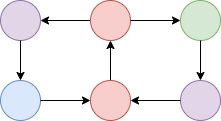
\includegraphics[scale=0.8]{images/contraction/before.png}
  \caption{A source graph before contraction}
\end{subfigure}
\begin{subfigure}{.5\textwidth}
  \centering
  % include second image
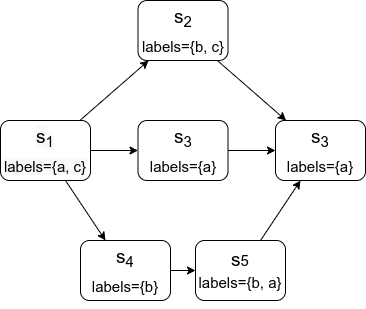
\includegraphics[scale=0.8]{images/contraction/after.png}
  \caption{The same source graph after contraction.}
\end{subfigure}
\caption{Contraction applied to a source graph. With this optimisation, 4 fewer vertices and edges need to be mapped. When mapping the downward edges of (b), checks are made to make sure that one path has a purple vertex followed by a blue vertex, and the other has a green vertex followed by a purple vertex.}
\label{fig:contraction}
\end{figure}

